\chapter{Proces detekcie anonymizovaných častí dokumentov}
\label{chap:FourthChapter}

\section{Algoritmy a techniky detekcie}
\begin{hyphenrules}{nohyphenation}
Všetky popisy algoritmov v sekcii \ref{chap:4.1.1} sú citované z knihy \textit{Počítačové videnie Detekcia a rozpoznávanie objektov}\cite{sikudova2014videnie}. V prípade, že citujeme z iného zdroja, bude tento zdroj explicitne referencovaný.
\subsection{Použité algoritmy}\label{chap:4.1.1}
%\todo[inline]{Ked beriete vsetky udaje z jedneho zdroja, tak to na zaciatku napiste a nemusite potom uvadzat citacie u kazdej zmienky}
Celý priebeh detekcie anonymizovaných oblastí je zložený na snahe redukovať čo naviac šumu a vyčistiť obraz tak, aby bolo jendoduché využiť za pomoci prahovania morfologické operácie dilatáciu a eróziu. 
\newline
\subsubsection{Morfologické operácie}
"\textit{Morfologické spracovanie obrazu využíva informáciu o susedných pixeloch v~topologickom okolí spracovávaného pixela.}"
Pre správne pochopenie fungovania týchto morfologických operácií je dôležité najprv zadefinovať tzv. štrukturálny element. Predtým však ešte spomenieme Minkowského sumu.

\begin{defn}{Minkowského suma}

    Minkowského suma bodových množín $A$ a $B$ je bodová množina
    \[C = \bigcup_{b\in B}A_b\]
kde

$A_b$ je množina $A$ posunutá o vektor $b$, teda množina $A_b = a + b | a \in A$. $\bigcup$ označuje zjednotenie (union) množín.
Minkowského sumu množín $A$ a $B$ označujeme
\[C = A \oplus B\]
\end{defn}
\subsubsection{Štrukturálny element}

Štrukturálny element $S$ je bodová množina s veľkosťou menšou než vstupný obraz. Jeho typický rozmer býva pomerne malý, napr. $3\times3, 5\times5,\dots21\times21$ atď. V Minkowského sume je vstupný obraz označený $A$ a štrukturálny element je tu označený ako $B$.
\newline

Morfologickú transformáciu je možné definovať ako matematickú reláciu medzi dvomi bodovými množinami, a to množinou obrazu a množinou použitého štrukturálneho~elementu.
\begin{defn}{Dilatácia}

    Operáciu binárnej dilatácie spracovávaného obrazu $A$ a štrukturálneho elementu $S$ značíme
    \[A\oplus S.\]
    Binárna dilatácia vyplýva z uvedenej definície Minkowského sumy zjednotenia posunutých bodových množín $A$ a $S$. Binárnu dilatáciu môžeme zapísať ako
    \[A \oplus S = \bigcup_{s \in S} A_s,\]
    kde $A_s$ je množina $A$ posunutá o vektor $s$, teda množina
    \[A_s = a + s | a\in A.\]
\end{defn}

\begin{defn}{Erózia}

    Operáciu erózie spracovávaného obrazu $A$ a štrukturálneho elementu $S$ značíme
    \[A\ominus S.\]
    Binárnu eróziu môžeme zapísať ako prienik všetkých posunov obrazu $A$ o vektory $-s$, kde $s \in S$:
    \[A \ominus S = \bigcap_{s \in S} A_s,\]
    kde $A_s$ je množina $A$ posunutá o vektor $s$, teda množina
    \[A_s = a + s | a\in A.\]
\end{defn}

\begin{figure}[H]
    \centering
    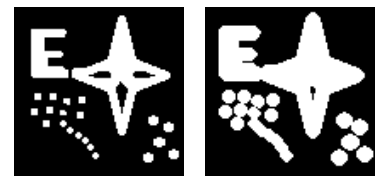
\includegraphics[width=0.5\linewidth]{img/dilatacia.png}
    \caption{Vľavo je vstupný obraz, vpravo dilatovaný výstupný obraz.}
    \label{fig:dilate}
\end{figure}
\begin{figure}[H]
    \centering
    
\includegraphics[width=0.5\linewidth]{img/erozia.png}
    \caption{Vľavo je vstupný obraz, vpravo erodovaný výstupný obraz.}
    \label{fig:erode}
\end{figure}
\subsubsection{Morfologické otvorenie a uzavretie}
Nosnými operáciami použitého algoritmu na detegovanie anonymizovaných oblastí sú využitia kombinácií dilatácie a erózie. 
\subsubsection{Morfologické otvorenie}
    
    Pod morfologickým otvorením rozumieme použitie erózie a následne dilatácie. Túto operáciu môžeme zapísať ako
    \[(A\ominus S) \oplus S. \]
    
\subsubsection{Morfologické uzavretie}
    
    Pod morfologickým uzavretím rozumieme použitie dilatácie a následne erózie, teda v opačnom poradí. Túto operáciu môžeme zapísať ako
    \[(A\oplus S) \ominus S. \]
    
\begin{figure}[H]
    \centering
    
\includegraphics[width=0.5\linewidth]{img/otvorenie.png}
    \caption{Vľavo je vstupný, vpravo výstupný obraz po operácii morfologického otvorenia.}
    \label{fig:open}
\end{figure}
\begin{figure}[H]
    \centering
    
\includegraphics[width=0.5\linewidth]{img/uzavretie.png}
    \caption{Vľavo je vstupný, vpravo výstupný obraz po operácii morfologického uzavretia.}
    \label{fig:close}
\end{figure}
Všimnime si, aký efekt má použitie otvorenia, resp. uzavretia na vstupný obraz. Pri morfologickom otvorení na obrázku \ref{fig:open} vidíme, že sú odstránené malé izolované oblasti, resp. oblasti, ktoré sú tenké a menšie než použitý štrukturálny element. Naopak, pri uzavretí (obr. \ref{fig:close}) vidíme "spájanie" izolovaných častí, ktoré sú dostatočne blízko seba, aby boli pokryté štrukturálnym elementom. Výsledný obraz je teda veľmi ovplyvnený tým, aký tvar, resp. aký veľký je použitý štrukturálny element. 

\subsubsection{Prahovanie}
    
Prahovanie je jednoduchý koncept, kde na základe určených parametrov ohraničíme intenzitu jednotlivých pixelov. V prípade šedotónového obrazu, kde má každý pixel hodnotu od 0 do 255, ak použijeme prahovanie, napr. horný prah 150 a spodný prah 20, všetky pixely vo výslednom obraze budú v tomto rozmedzí, a teda pixely s hodnotou nižšou než 20 sa nastavia na 20 a naopak, pixely s hodnotou vyššou než 150 sa nastavia na 150.
\newline

Na prahovanie využívame OTSU algoritmus\cite{otsu}, ktorý je založený na princípe hľadania najlepšej hodnoty prahu na rozdelenie obrázka na tmavé a svetlé časti tak, aby bol rozdiel medzi nimi čo najväčší.
\newline

Na filtráciu šumu a detekciu hľadaných oblastí sme vyskúšali aj tzv. korekciu neuniformného osvetlenia\cite{plantcv}, každopádne výsledky boli na našich testovacích dátach zhodné s použitím kombinácie vyššie spomenutých morfologických operácií.

\subsection{Zvolená kombinácia algoritmov}
\label{chap:4.1.2}
%\todo[inline]{Tuto trochu upravte nazvy casti 1 a 2}
Po niekoľkých iteráciách, ktoré sú popísané v ďalšej podkapitole, sme pristúpili na finálny algoritmus pozostávajúci z prahovania a následnej kombinácie viacnásobného použitia dilatácie a erózie. To nám umožnilo efektívne odstrániť šum a text, ktorý sa v dokumentoch vyskytoval a výsledným obrazom boli anonymizované oblasti. V prípade, že bola detegovaná farba v obrázku, pracovali sme s variantom, že sa jedná o typ anonymizácie farebnou nálepkou a týmto farebným pixelom sme zmenili farbu na fialovú a zvýšili saturáciu tak, aby boli jednoznačne identifikovateľné. Fialová farba bola zvolená z dôvodu, že sa v~skúmaných dokumentoch táto farba nikde nevyskytovala. 
%\todo[inline]{skuste popisat aj ake prahovanie pouzivate}
\newline

Celý algoritmus je zložený nasledovne:
V prvom kroku zistíme či je obraz šedotónový alebo obsahuje nejaké farebné pixely. Ak obraz má nejaké farebné pixely, tieto pixely saturujeme. Následne obraz dilatujeme východzím štvorcovým štrukturálnym elementom o veľkosti 3$\times$3 pixely z knižnice OpenCVSharp\cite{opencv}. Po dilatácii obraz prahujeme a následne opakovane dilatujeme. Vďaka viacnásobnej dilatácii sa nám spoja izolované pixely, vďaka čomu sme schopní následne viacnásobne erodovať, čím odstraníme šum a aj väčšinu textu. Po viacnásobnej erózii znovu dilatujeme, aby sme vykompenzovali stratu pixelov na hranách oblastí, ktoré chceme detegovať, pre lepší výpočet pomeru oblastí vzhľadom na celú stranu. Výsledkom je obraz, ktorý obsahuje len hľadané anonymizované oblasti (obr. \ref{fig:4.5}).

\begin{figure}[H]
\begin{minipage}[t]{.4\linewidth}
\fbox{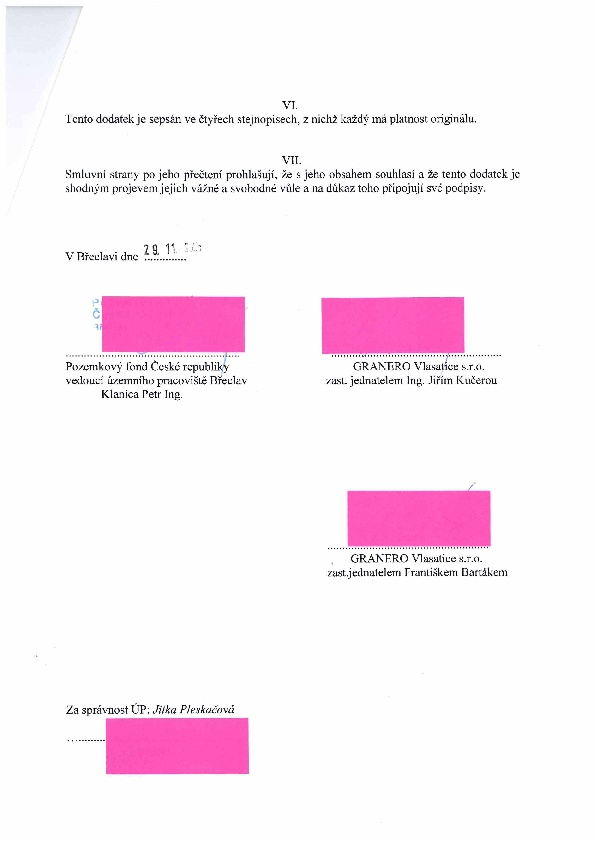
\includegraphics[width=0.9\linewidth]{img/3_original.jpg}}
\caption{Vľavo vstupný obraz, vpravo výstupný.}
\label{fig:4.5} 
\end{minipage}\hfill
\begin{minipage}[b]{.4\linewidth}
\fbox{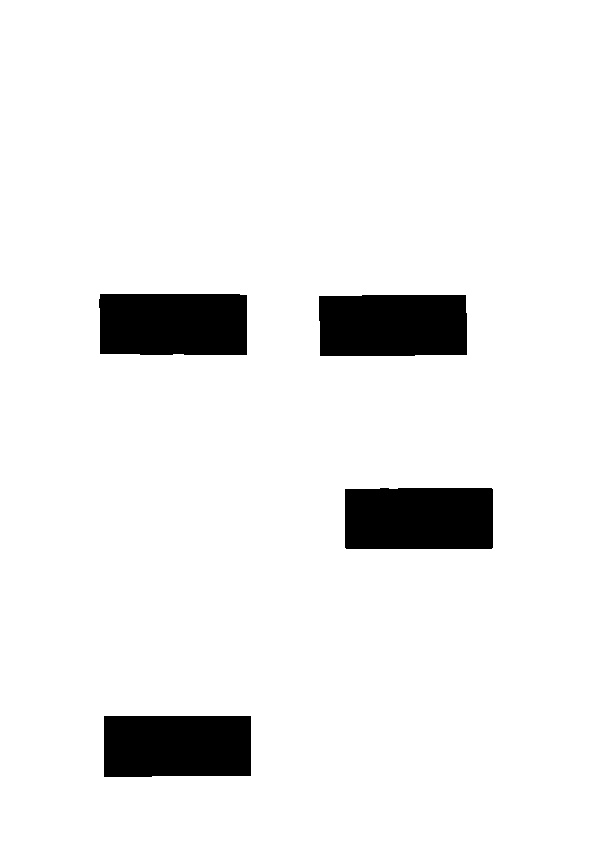
\includegraphics[width=0.9\linewidth]{img/3_result.jpg}}
\end{minipage}
\end{figure}

Tento algoritmus je schopný detegovať aj typ anonymizácie, kde je použitý šum, avšak nie úplne dokonale (obr. \ref{fig:4.6}).
\begin{figure}[H]
\begin{minipage}[t]{.4\linewidth}
\fbox{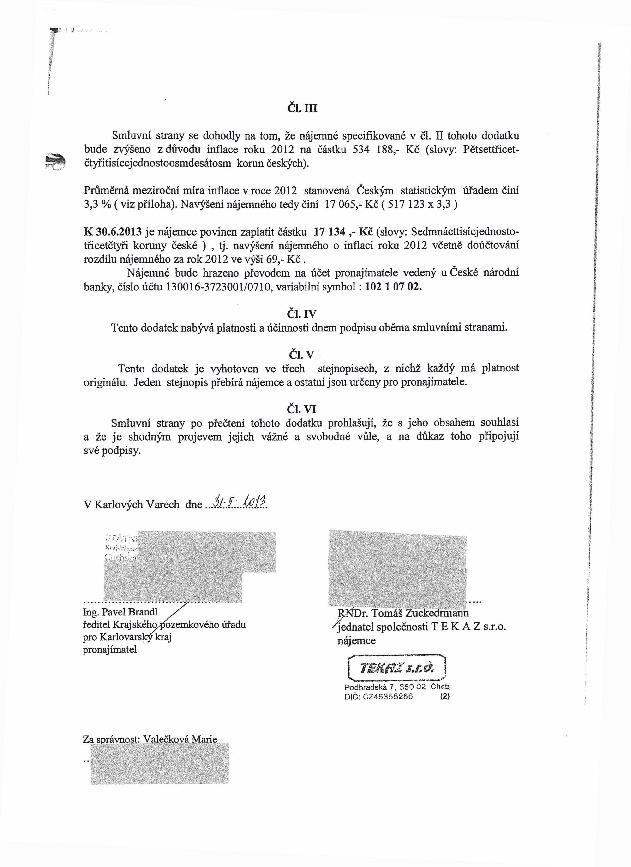
\includegraphics[width=0.9\linewidth]{img/2_original.jpg}}
\caption{Vľavo vstupný obraz, vpravo výstupný.}
\label{fig:4.6} 
\end{minipage}\hfill
\begin{minipage}[b]{.4\linewidth}
\fbox{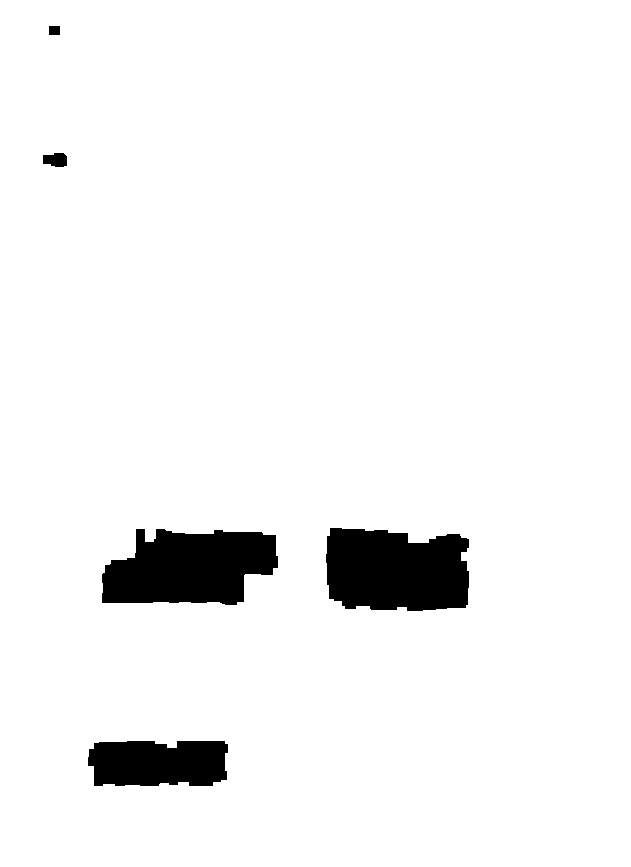
\includegraphics[width=0.9\linewidth]{img/2_result.jpg}}
\end{minipage}
\end{figure}

\subsection{Výpočet anonymizácie}
Na záver vypočítavame celkové percento pokrytia anonymizovanej oblasti relatívne k obsahu strany. Keďže neexistuje jednoznačne najlepšia metrika, podľa čoho takéto percento počítať, rozhodli sme sa, že použijeme nasledovný výpočet: 

V originálnom obraze spočítame nenulové pixely, teda len pixely, ktoré nesú nejakú informáciu 
(časť písmena textu, tabuľka. . . ) a touto hodnotou predelíme počet pixelov, ktoré sme na analyzovanej 
strane detegovali ako anonymizované oblasti, prenásobené koeficientom, keďže je zjavné, že nie celá 
prekrytá časť obsahuje relevantné informácie.
\newline

Pretože informácie prekryté anonymizovanou oblasťou sú dôležité, je potrebná ich kompenzácia 
vhodným koeficientom. Pri analýze a testovaní sme zvolili ako najvhodnejšiu hodnotu kompenzačného 
koeficientu 0.83. Výsledná hodnota je v~rozsahu od 0 do 1, a teda percento údajov, ktoré boli 
anonymizované.
\newline

Väčšinou sa však jedná len o podpisy alebo mená, preto sa výsledné hodnoty pohybujú zväčša v rozmedzí od 0.01 do 0.10. Napríklad výsledná hodnota pre vyššie zobrazené výstupy (obr. \ref{fig:4.5}) je 0.064, a teda 6,4\%, (obr. \ref{fig:4.6}) je to 0.042, resp. 4,2\%.
\section{Validácia a testovanie}
\subsection{Testovacie stratégie}
Keďže sme nemali k dispozícii referenčné riešenie, oproti ktorému by sme mohli porovnať naše výsledky, zvolili sme stratégiu, ktorá zarhňovala manuálne porovnávanie a empirické odhady správnosti. Výsledky sme porovnávali v~rámci vybraného datasetu siedmich dokumentov, ktorý obsahoval ako skenované, tak digitálne dokumenty spoločne so všetkými nájdenými typmi anonymizácie.
\newline 

Na generáciu výsledkov bol vytvorený projekt \texttt{GenerateTestResults}, vďaka ktorému sme mohli pozorovať zmeny vzhľadom na jednotlivé úpravy. Mimo kontroly správnosti samotných výsledkov sme aplikáciu pokryli unit a integračnými testami, aby sme zaručili správnosť a funkčnosť aj v prípade nevalidných dokumentov či zlyhania siete, v prípade sťahovania dokumentov cez internet.

\subsection{Analýza výsledkov a iteratívne zlepšovanie}
Prínosom v práci bola možnosť iteratívne skúmať rôzne kombinácie skladania morfologických operácií, vďaka čomu sme boli schopní prísť s najlepšou možnou kombináciou v rámci relatívne objektívneho hodnotenia detekcie oblastí.
\end{hyphenrules}